\chapter{Аналитическая часть} \label{chapt1}

\section{Основные понятия теории компиляции} \label{sec11} 

\subsection{Компилятор} \label{sub111}

Компилятор~--- это программа, которая  принимает текст, написанный на~одном языке~--- \textit{исходном}, и~транслирует (переводит) его в~эквивалентный текст на~другом языке~--- \textit{целевом}~\cite{Aho2003}. Процесс компиляции можно разделить на~две части.

 Первая часть~--- \textit{анализ} (выполняется в несколько фаз) разбивает исходную программу на~составные части и~накладывает на~них грамматическую структуру. Затем эта структура используется для генерации промежуточного представления программы. Анализатор сообщает пользователю об~ошибках, собирает информацию об~исходной программе и~сохраняет в~\textit{таблицу символов}. Таблица символов~--- структура данных, которая используются компилятором для хранения информации о~конструкциях исходной программы. Информация накапливается инкрементно в~фазе анализа компилятора и~используется фазой синтеза для генерации целевого кода.

Вторая часть~--- \textit{синтез} (выполняется генератором кода), строит требуемую целевую программу на~основе промежуточного представления и~информации из~таблицы символов.

Анализ и синтез делятся на несколько шагов, которые представлены на~рис.~\ref{img:compiler-structure-2}.

\begin{figure}[ht]
	\centering
	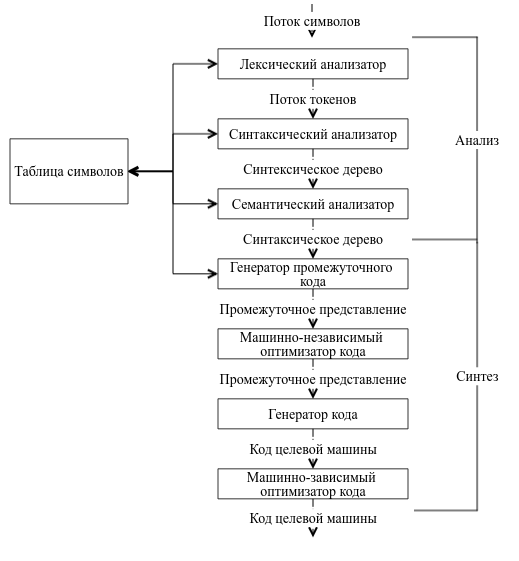
\includegraphics [scale=0.75] {compiler-structure}
	\caption{Схема взаимодействия фаз компилятора}
	\label{img:compiler-structure-2}
\end{figure}

Анализ:
\begin{itemize}
\item{\textit{Лексический анализ} или \textit{сканирование}. Лексический анализатор читает поток символов, составляющих исходную программу, группирует их в~значащие последовательности (лексемы), формирует для каждой лексемы специальные структуры данных, называемые токенами, и~передает их синтаксическому анализатору.}	
\item{\textit{Синтаксический анализ} или \textit{разбор}. Синтаксический анализатор использует информацию из предыдущей фазы и~на её основе строит синтаксическое дерево, в~котором каждый внутренний узел представляет операцию, а~дочерние узлы~--- аргументы этой операции.}	
\item{\textit{Семантический анализ}. Эта фаза компиляции использует синтаксическое дерево и~информацию из таблицы символов для проверки исходной программы на семантическую согласованность с~определением языка. Важной частью семантического анализа является проверка и~приведение типов.}
\end{itemize}

Синтез:
\begin{itemize}	
\item{\textit{Генерация промежуточного кода.} На этой фазе компилятор генерирует низкоуровневое промежуточное представление кода исходной программы, которое можно рассматривать как программу для абстрактной вычислительной машины.}	
\item{\textit{Машинно-независимая оптимизация кода.} Фаза машинно-независимой оптимизации кода пытается улучшить промежуточный код. Например, заменить вызов метода на~непосредственное выполнение тела метода в~месте вызова.}	
\item{\textit{Генерация кода.} В качестве исходных данных генератор кода получает промежуточное представление исходной программы и~отображает его в~целевой язык, как правило в~ассемблерный код.}
\item{\textit{Машинно-зависимая оптимизация кода.} Фаза машинно-зависимой оптимизации кода улучшает код целевой машины, учитывая особенности архитектуры процессора.}		
\end{itemize}


Процесс анализа компиляции разделен на~лексический, синтаксический и~семантический анализ по~ряду причин: 

\begin{enumerate} 
	\item{Упрощение разработки. Отделение лексического анализа от~синтаксического позволяет упростить как минимум одну из~фаз анализа. Например, удаление комментариев и~пробельных символов лексическим анализатором значительно проще, чем включение работы с~ними в~синтаксический анализатор.}
	\item{Увеличение переносимости компилятора. Например, для того, что~бы~компилятор работал на~разных операционных системах достаточно реализовать только часть генерации кода, вместо написания второго компилятора.}
	\item{Разделение зон ответственности. Каждый компонент отвечает только за определённую часть функциональности. Таким образом сокращается вероятность допущения ошибки, код каждого компонента становится легко модифицируемым. }
\end{enumerate}

\subsection{Лексический анализатор} \label{sub112}

При рассмотрении лексического анализа используются три термина:

\begin{itemize} 
	\item{
		\textit{Токен} (от~англ. \textit{token}~--- знак, символ) представляет собой пару, состоящую из~имени токена и~необязательного атрибута. Имя токена~--- абстрактный символ, представляющий тип лексической единицы, например, конкретное ключевое слово или последовательность символов, составляющих идентификатор. Имена токенов являются входными символами, обрабатываемыми синтаксическим анализатором. Атрибут токена~--- строка или структура, объединяющая несколько блоков информации описание лексемы (строчка кода, значение), которая представляет токен. 
		Выражение на~языке Fortran \texttt{E=M*2} будет представленно в~виде последовательности \\
		$\bnfpn{\textbf{id}, Указатель на запись в таблице символов для E}$ \\
		$\bnfpn{\textbf{assign\_op}}$ \\
		$\bnfpn{\textbf{id}, Указатель на запись в таблице символов для M}$ \\
		$\bnfpn{\textbf{mult\_op}}$ \\
		$\bnfpn{\textbf{number}, Целое значение 2}$ \\
		Примеры токенов приведены в~табл.~\ref{tokens}.
		\begin{table} [h!tbp]
			\centering
			\changecaptionwidth\captionwidth{15.35cm}
			\caption{Примеры токенов}\label{tokens}%
			\begin{tabular}{| p{3cm} | p{6cm} | p{5cm} |} \hline
				\textbf{Токен}		&	\textbf{Неформальное описание}												&	\textbf{Примеры лексем}						\\ \hline
				\textbf{if}  		& 	Символы \texttt{i}, \texttt{f} 												& 	\texttt{if} 								\\ \hline
				\textbf{else}  		& 	Символы \texttt{e}, \texttt{l}, \texttt{s} \texttt{e} 						& 	\texttt{else} 								\\ \hline
				\textbf{comparison}	& 	\texttt{<}, \texttt{>}, \texttt{<=}, \texttt{>=}, \texttt{==}, \texttt{!=}	& 	\texttt{<=}, \texttt{!=} 					\\ \hline
				\textbf{id}  		& 	Буква, за~которой следуют буквы и~цифры										& 	\texttt{pi}, \texttt{score}, \texttt{D2}	\\ \hline
				\textbf{number}  	& 	Любая числовая константа													& 	\texttt{3.14159}, \texttt{0} 				\\ \hline
				\textbf{literal}  	& 	Все, кроме \texttt{"}, заключенное в~двойные кавычки 						& 	\texttt{"core dumped"} 						\\ \hline	
			\end{tabular}
		\end{table}	
	}
	\item{\textit{Шаблон}~--- это описание вида, который может принимать лексема токена. В~случае ключевого слова шаблон представляет собой последовательность символов, образующая это ключевое слово. Для некоторых токенов шаблон представляет более сложную структуру (регулярное выражение).}
	\item{\textit{Лексема}~--- последовательность символов исходной программы, которая соответствует шаблону токена и~идентифицируется лексическим анализатором как экземпляр токена.}
\end{itemize}

Основная задача лексического анализатора~--- чтение входных символов исходной программы, группировка их ~в~лексемы и~вывод последовательностей токенов для всех лексем исходной программы. Поток токенов пересылается синтаксическому анализатору для разбора. Лексический анализатор удаляет комментарии, пробельные символы, синхронизирует сообщения об~ошибках и раскрывает макросы.
\subsection{Формальное определение контекстно-свободной грамматики} \label{sub114}

Для работы синтаксического анализатора требуется описание грамматики языка программирования, которое задаётся с помощью контекстно-свободных грамматик (далее КС-грамматики).

Существует множество типов грамматик (грамматики типа~3, контекстно-свободные грамматики, контекстно-зависимые грамматики и грамматики без ограничений), с~помощью которых можно описать различные языки. Для описания языков программирования используются КС-грамматики, потому что их разбор наиболее быстрый.

КС-грамматика используется для определения формального синтаксиса языка программирования. КС-грамматика естественным образом описывает иерархическую структуру множества конструкций языка программирования. Ниже приведён пример КС-грамматики, которая описывает выражение \texttt{switch} языка \texttt{Java}:
\begin{align*}
SwitchStatement &\to \textbf{switch}\;\textbf{(}\; Expression\; \textbf{)}\; SwitchBlock \\
SwitchBlock &\to \textbf{\{}\; \textbf{\{}\;SwitchBlockStatements\;\textbf{\}}\; \textbf{\{}\;SwitchLabel\;\textbf{\}}\; \textbf{\}} \\
SwitchBlockStatements &\to SwitchLabels\; BlockStatements \\
SwitchLabels &\to SwitchLabel\; \textbf{\{}\;SwitchLabel\;\textbf{\}} \\
SwitchLabel &\to \textbf{case}\; ConstantExpression\; \textbf{:} \\
SwitchLabel &\to \textbf{case}\; EnumConstantName \;\textbf{:} \\
SwitchLabel &\to \textbf{default\;:} \\
EnumConstantName &\to Identifier \\
ConstantExpression &\to Expression
\end{align*}

КС-грамматика состоит из~четырёх частей:
 
\begin{enumerate} 
	\item{\textit{Терминалы}~--- базовые символы, формирующие строки. Термин <<Имя токена>> является синонимом слова <<Терминал>>. Пример терминала: \texttt{switch}, \texttt{case}, \texttt{(}, \texttt{)}}. Другими словами, это листья дерева разбора, представленного на~рис.~\ref{img:tree}.
	\item{\textit{Нетерминалы}~--- синтаксические переменные, которые обозначают множества строк. В~примере, приведённом выше, $\begin{aligned} Expression \end{aligned}$, $\begin{aligned} SwitchBlock \end{aligned}$, $\begin{aligned} SwitchLabel \end{aligned}$ и~др. являются нетерминалами. Эти множества строк, обозначаемые нетерминалами, помогают определить язык, порождаемый КС-грамматикой. Нетерминалы также налагают на~язык иерархическую структуру, облегчающую синтаксический анализ и~трансляцию.}
	\item{\textit{Стартовый символ}~--- один из~нетерминалов, который обозначает множество строк, определяемых КС-грамматикой. По~соглашению, продукции стартового символа указываются первыми (в примере это $\begin{aligned} SwitchStatement \end{aligned}$).}
	\item{\textit{Продукция}~--- способ, которым терминалы и~нетерминалы объединяются в~строки. Каждая продукция состоит из~заголовка (левая часть), символа $\begin{aligned} &\to \end{aligned}$ и~тела (правая часть), которое состоит из~нуля или некоторого количества терминалов и~нетерминалов.}
\end{enumerate}
 
\subsection{Синтаксический анализатор} \label{sub113}

В~классической модели компилятора синтаксический анализатор получает строку токенов от~лексического анализатора и~проверяет, может ли~эта строка имен токенов порождаться грамматикой исходного языка. Также от~синтаксического анализатора ожидаются сообщения обо~всех выявленных ошибках и~умение продолжать работу с~оставшейся частью программы. В~случае корректной программы синтаксический анализатор строит дерево разбора и~передает его следующей части компилятора для дальнейшей обработки.

Имеется три основных типа синтаксических анализаторов грамматик: 

\begin{itemize} 
	\item{\textit{Универсальные методы разбора}, например, алгоритмы Кока-Янгера-Касами (Cocke-Younger-Kasami) и~Эрли (Earley)\cite{Earley1983} могут работать с~любой грамматикой. Однако эти обобщённые методы слишком неэффективны для использования в~промышленных компиляторах. }
	\item{\textit{Восходящие методы разбора} (bottom-up), построение дерева разбора происходит снизу (от~листьев) вверх (к~корню). Поток токенов сканируется слева направо. }
	\item{\textit{Нисходящие методы разбора} (top-down) строят дерево разбора сверху (от~корня) вниз (к~листьям). Входной поток синтаксического анализатора, как и~в~восходящих методах, сканируется посимвольно слева направо. }
\end{itemize}

\todo{Пример выражения на языке программирования и соответствующее ему синтаксическое дерево.}

\subsection{Семантический анализатор} \label{sub115}

Семантический анализатор использует синтаксическое дерево и~информацию из~таблицы символов для проверки исходной программы на~семантическую согласованность с~определением языка. Он также собирает информацию о~типах и~сохраняет ее в~синтаксическом дереве или в~таблице символов для последующего использования в процессе генерации промежуточного кода.

Важной частью семантического анализа является проверка типов, когда компилятор проверяет, имеет ли~каждый оператор операнды соответствующего типа. Например, многие определения языков программирования требуют, чтобы индекс массива был целым неотрицательным числом. Компилятор должен сообщить об ошибке, если в~качестве индекса массива используется число с~плавающей точкой.
\subsection{Генератор лексических анализаторов Lex} \label{sub116}

\textit{Lex} (в~более поздних реализациях \textit{Flex})~--- программный инструмент, который позволяет определить лексический анализатор, указывая регулярные выражения для описания шаблонов токенов. Входные обозначения для Lex обычно называют \textit{языком Lex}, а~сам инструмент~--- \textit{компилятором~Lex}. Компилятор~Lex преобразует входные шаблоны в~диаграмму переходов~\cite{Levine1992}. 

На~рис.~\ref{img:lex} показанна схема использования генератора Lex. Входной файл \texttt{lex.l} написан на~языке Lex~и описывает генерируемый лексический анализатор. Компилятор Lex преобразует \texttt{lex.l}~в программу на~языке программирования~C в~файле с~именем \texttt{lex.yy.c}.  Этот файл преобразуется компилятором~C~в файл~с названием \texttt{a.out}. Результат работы компилятора~C~--- работающий лексический анализатор, реализующий восходящий анализ, который может получать поток входных символов~и выдавать поток токенов~\cite{Aho2003}.

\begin{figure}[ht]
	\centering
	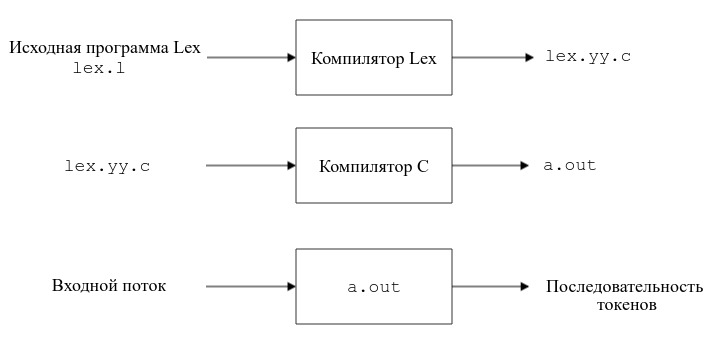
\includegraphics [scale=0.65] {lex}
	\caption{Создание лексического анализатора с~помощью Lex}
	\label{img:lex}
\end{figure}

Следующим поколением лексического генератора Lex стал \textit{Flex (Fast lex)}. Flex практически полностью совместим с Lex. Отличия Flex от~Lex:

\begin{itemize} 
	\item{может компилироваться в~C++, что позволяет использовать объектно-ориентированные конструкции~C++;}
	\item{генерирует более производительные лексические анализаторы;}
	\item{не~имеет ограничений по~размеру для таблиц символов (в~отличие от~Lex);}
	\item{небольшие синтаксические различия~\cite{Levine1992}. }
\end{itemize}

\subsection{Генератор синтаксических анализаторов Yacc} \label{sub117}

\textit{Yacc}~---компьютерная программа, служащая стандартным генератором синтаксических анализаторов в~Unix-системах. Название является акронимом \textit{<<Yet Another Compiler Compiler>>} (<<ещё один компилятор компиляторов>>)\cite{Johnson1975}. Yacc генерирует синтаксический анализатор на~основе аналитической грамматики, описанной в~нотации Бэкуса-Наура или контекстно-свободной грамматики. На выходе yacc выдаётся код на~языке программирования~Си.

Поскольку синтаксический анализатор, генерируемый с~помощью yacc, требует использования лексического анализатора, то~часто он используется совместно с~генератором лексических анализаторов, в~большинстве случаев это lex либо flex. 

\todo{Схема? Пример программы на yacc?}
\subsection{Универсальные генераторы анализаторов} \label{sub118}

Помимо инструментов, которые генерируют отдельно синтаксический и лексический анализаторы, существуют универсальные генераторы, способные автоматизировать создание лексического и синтаксического анализаторов одновременно. 

\textit{ANTLR}~--- генератор синтаксических и~лексических анализаторов. Реализует алгоритмы нисходящего анализа. Обладает развитыми возможностями по~оптимизации таблиц разбора. За счет чего достигается конкурентоспособность в~быстродействии конечного продукта против решений построенных на реализации восходящих алгоритмов анализа.
На вход принимается описание контекстно-свободной грамматики в~Расширенной форме Бекуса-Наура. На выход выдается код синтаксического и лексического анализаторов на~языках Java или~C++ и~других. Активно
используется во~многих продуктах, таких как среда разработки Eclipse, NetBeans, система баз данных Cassandra и~другие.

\textit{Coco/R}~--- генератор синтаксических и~лексических анализаторов. Реализует алгоритмы нисходящего рекурсивного анализа. На~вход принимается описание контекстно-свободной грамматики в~Расширенной форме Бекуса-Наура. На~выход выдается код синтаксического и лексического анализаторов на~языках Java, C++ или~других~\cite{dskMag}.

\section{Предметно-ориентированные языки программирования} \label{sec12}
\subsection{Определение предметно-ориентированного языка программирования} \label{sub121}

\textit{Предметно-ориентированный язык программирования (domain-specific language, DSL)}~--- язык программирования или исполняемая спецификация, которые предлагают выразительное и~мощное решение конкретной предметной проблемы с~помощью высокоуровневых абстракций и~специализированных нотаций. Чаще всего такой язык программирования не~является большим и~предоставляет только те~конструкции, которые необходимы для решения предметной задачи (например, язык Yacc).

Альтернативой предметно-ориентированному языку является использование объектно-ориентированного языка программирования вместе с~библиотекой типов и~функций, которые отвечают предметным потребностям.~\cite{Deursen1998}
\subsection{Инструменты разработки предметно-ориентированных языков программирования} \label{sub122}
\todo{Тут будут разные языки программирования и инструменты (Kotlin, Scala, Groovy), с помощью которых можно создавать п-о яп. Будут приведены плюсы и минусы данных подходов. В том числе, среди минусов Groovy я отмечу плохую поддержку IDEA и отсюда вытечет формулировка задачи.}

\section{Поддержка DSL в современных редакторах кода} \label{sec13}
\subsection{Платформа IntelliJ} \label{sub131}

\textit{IntelliJ} ~--- платформа с~открытым исходным кодом для создания интегрированных сред разработки, которые включают в~себя:

\begin{itemize}
\item{виртуальную файловую систему;}
\item{поддержку визуального взаимодействия с пользователем;}	
\item{текстовый редактор;}	
\item{лексический и синтаксический анализ, с поддержкой различных языков программирования;}
\item{инструменты для реализации навигации, авто-дополнения исходного кода, рефакторинга и т.д.;}
\item{систему контроля версий;}
\item{инструменты для отладки приложений;}
\item{графическую поддержку запуска тестов.}
\end{itemize}

Самым популярным продуктом, который построен на основе платформы IntelliJ является IntelliJ~IDEA.

\textit{IntelliJ~IDEA}~--- интегрированная среда разработки программного обеспечения для многих языков программирования, в~частности Java, JavaScript, Python, разработанная компанией JetBrains. Помимо работы~с перечисленными языками, IntelliJ~IDEA предоставляет обширный инструментарий для поддержки языков программирования, включая DSL.
\subsection{Поддержка предметно-ориентированных языков программирования в IntelliJ IDE} \label{sub132}

Поддержка языка~--- процесс лексического, синтаксического и~семантического анализа c целью навигации, автодополнения и подсветки синтаксиса исходного кода, написанного на поддерживаемом языке программирования. 

Для реализации поддержки различных языков программирования платформа IntelliJ предоставляет возможность добавления собственных лексических и синтаксических анализаторов с последующей интеграцией с~IntelliJ.

Платформа IntelliJ преобразует исходный код в \textit{PSI(Program Structure Interface)}. PSI~--- набор функциональных возможностей, который предназначен для анализа файлов, построения синтаксических моделей исходного кода и создания индексов. Функциональные возможности PSI включают в себя:

\begin{itemize}
\item{быструю навигацию по файлам;}
\item{подсветку синтаксиса;}
\item{динамические проверки кода;}
\item{исправление кода, включая обширный рефакторинг;}
\item{автодополнение кода и д.р.}
\end{itemize}

Поддержка языка DSL, в~частности внутреннего, отличается от стандартной поддержки языка программирования общего назначения. Отличие заключается в том, что лексический и синтаксический анализ уже проведены для расширяемого языка программирования. Разработка модуля поддержи языка DSL сводится к правильному использованию уже готовых компонентов (PSI).
